\section{Introduction}
During the last years the usage of smart-wearables (particularly smartwatches) has become more and more common with a number of 337 million units sold in 2019 and a forecast in sales of up to 527 million units by 2024 \cite{tenzer}.
With that also comes a natural demand in data protection caused by the many sensors built in these devices and their ability to capture sensible personal information (e.g. health informations).
Additionally smart devices can now also be used for many kinds of financial actions.
Since most wearables are connected to either the distributors or the respective mobile phones virtual assistant they should contain sensors for on one hand sound conduction and on the other hand audio recording.
In the current general smart-wearable design neither of these sensors is oriented towards the wearers arm.
With a change in position of these sensors smartwatches become eligible for functional biometric authentication.
Further motivation for this new authentication method comes from the fact that the previous classical methods (PIN, password...) are not suited for usage on smartwatches \cite{xu2017gait}.   
Nevertheless it is shown by Johnston \cite{johnston2015smartwatch} and Yang \cite{yang2015motionauth} in their respective works that there already are potential biometric authentication methods for smartwatches based on distinct hand or arm movements. 

From these preconditions a prototype is defined. This prototype uses a sound based functional biometric which gets applied to its wearers arm. 

\section{Related Work}
This section will give an overview on the terms of biometrics and its variations, authentication and also what defines an authentication system.
Additionally an insight into other works on biometric or smartwatch based authentication will be provided. 

\subsection{Authentication}
The term in general describes the process based on which a security systems tries to approve someone's claim of identity \cite{bhattacharyya2009biometric}.
Based on the input type of this claim the term authentication can be further subdivided into explicit and implicit authentication.
\textit{Explicit} authentication is more often also known as traditional authentication \cite{ranjan2016automatic}.
This includes providing knowledge like PIN or password, using a token but also performing gestures, fingerprints etc. from the biometrical field.

\textit{Implicit} authentication on the other hand describes mechanisms where a user does not provide a password, etc. directly.
Instead users are authenticated based on observations of their behavioural patterns\cite{jakobsson2009implicit}.
These observations are qualified for the use in e.g. biometrics since every individual has its own distinct habits which could be captured and analysed using different sensors \cite{shi2010implicit}.
Furthermore Shi, Jakobsson et al. state in their 2009 and 2010 works that implicit authentication is well suited for usage in combination with mobile smart-devices \cite{shi2010implicit} or portable computers \cite{jakobsson2009implicit}.
Based on this they propose three different application scenarios.
First as a second factor in combination with passwords, second as the main authenticator and thus replacing the usage of a password and last as additional assurance or an extra trust factor when performing e.g. financial actions on a mobile device.

\subsection{Biometrics}
\textit{Biometrics} (as in the Greek terms \textit{bios} and \textit{metrikos}) describes the utilization of an individuals physical traits or behaviour to clearly identify one from others. Contrary to the more known verification methods of PINs, passwords or ID-cards biometric identification does not rely on tokens or knowledge which could easily be forgotten or stolen, rather than unique personal traits like fingerprints, face geometry or the specific way someone interacts \cite[chpt. 1.1]{jain2007handbook}\cite{delac2004survey}.
Depending on the concept of usage a biometric system can be used in either verification or identification mode \cite[chpt. 1.3]{jain2007handbook}.
These two modes can also be differed by the use of \textit{positive} or \textit{negative identification} techniques \cite{wayman2005introduction}.

As already stated above biometric authentication uses an individuals personal traits as authentication tokens. Based on the kind of trait and the methods how they are provided the general term of biometrics can be further divided into behavioural and physiological biometrics.
Also a new kind of biometrics called functional biometrics was introduced by Liebers and Schneegass in 2020 \cite{schneegass2020functbiometric}.

\subsubsection{Behavioural Biometrics}
Behavioural biometrics refers to authentication systems in which the process of authentication is related to the behaviour of an individual \cite{bhattacharyya2009biometric}.
In most cases this process is conducted with the use of primarily gestures or other actions or movements capable of being performed in everyday life \cite{yampolskiy2008behavioural}.
Features which can be used for behavioural biometrics include e.g gait, keystrokes but also authentication patterns on smartphones could be used.
One main advantage compared to physiological biometrics is that some behavioural traits must not be collected actively but can be captured whilst performing any kind of different tasks \cite{yampolskiy2008behavioural}. 
Also there is no definite need for special hardware since the sensors needed are mostly built in smart wearables which are one of the main users of behavioural biometrics \cite{johnston2015smartwatch}.

\subsubsection{Physiological Biometrics}
Apart from behavioural biometrics the classification of physiological biometrics is also existent. 
This form of biometric authentication uses the more "static" traits of a users body as token such as e.g. fingerprints, hand geometry \cite{alsaadi2015physiological} or vein patterns \cite{faltaous2019vpid}.

A physiological system should also have a little higher accuracy than a behavioural one and it should be harder to use as an imposter since it is nearly impossible to identically copy a finger print, iris pattern, etc. \cite{koong2014user}, \cite{delac2004survey}.

\subsubsection{Functional Biometrics} With functional biometrics another novel kind of biometric authentication was introduced lately by Liebers and Schneegass \cite{schneegass2020functbiometric}.
This new concept stands as a major influence to this work notably with its first implementation in SkullConduct\cite{SkullConduct}. 
\begin{figure}
	\begin{center}
		\subfloat[Traditional Biometrics]{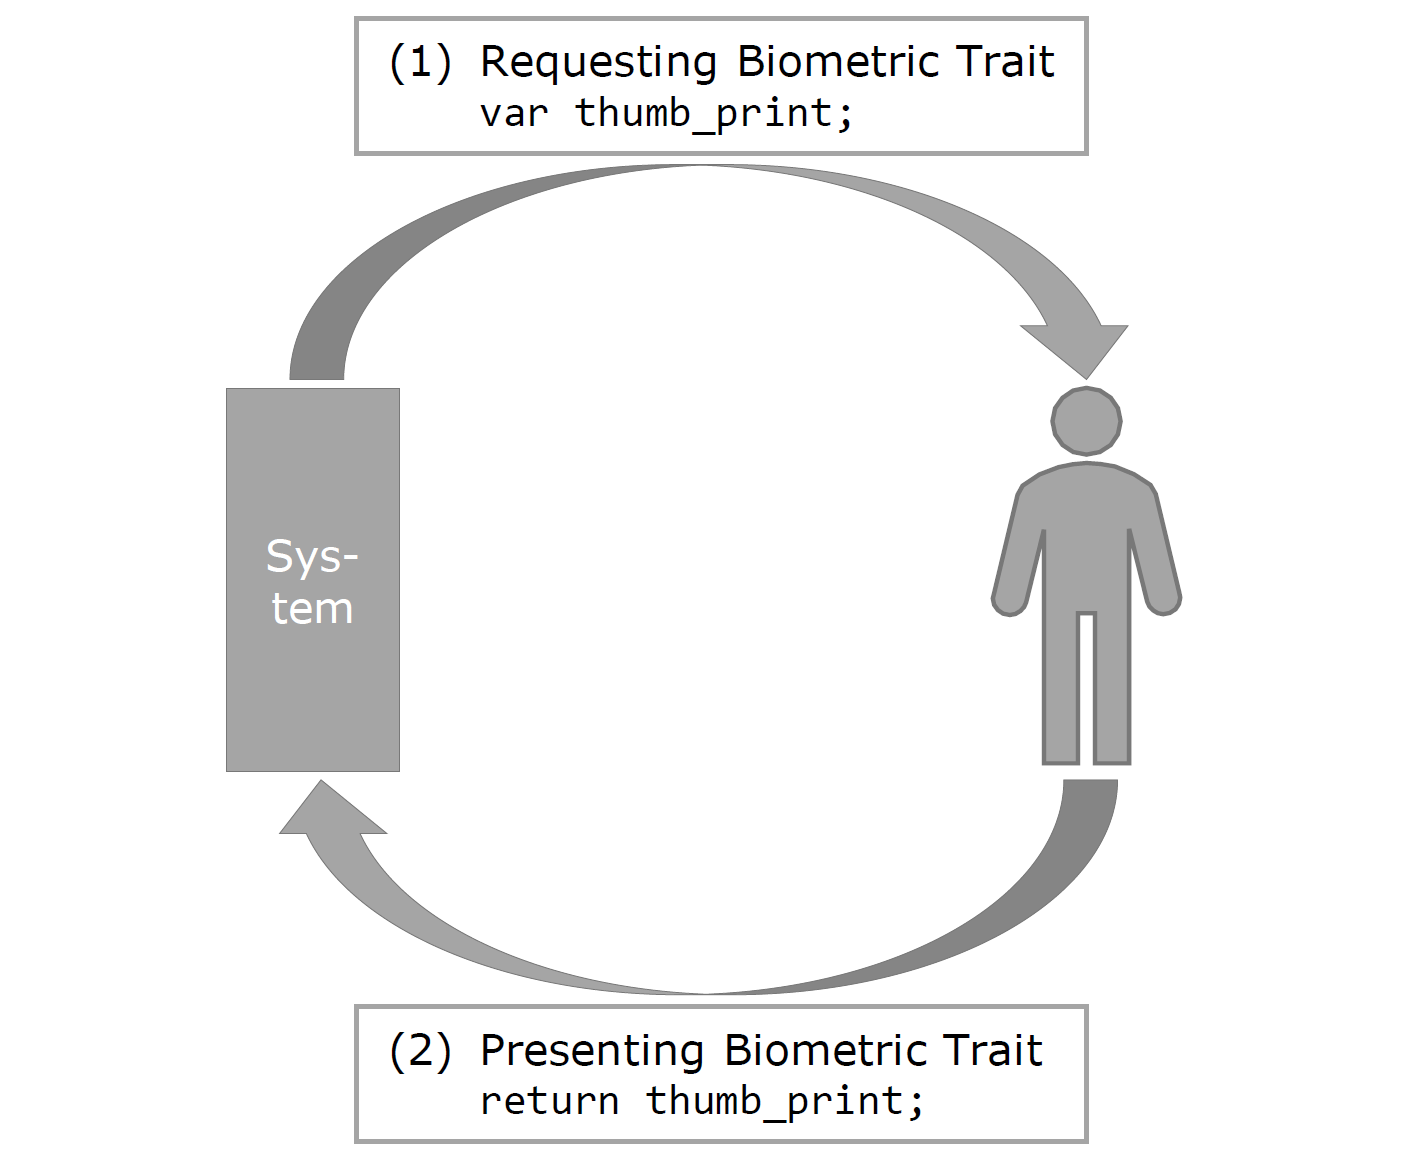
\includegraphics[width=0.4\textwidth]{biometric_trad.png}\label{fig:tradBiom}}
		\hspace{0.5cm}
		\subfloat[Functional Biometrics]{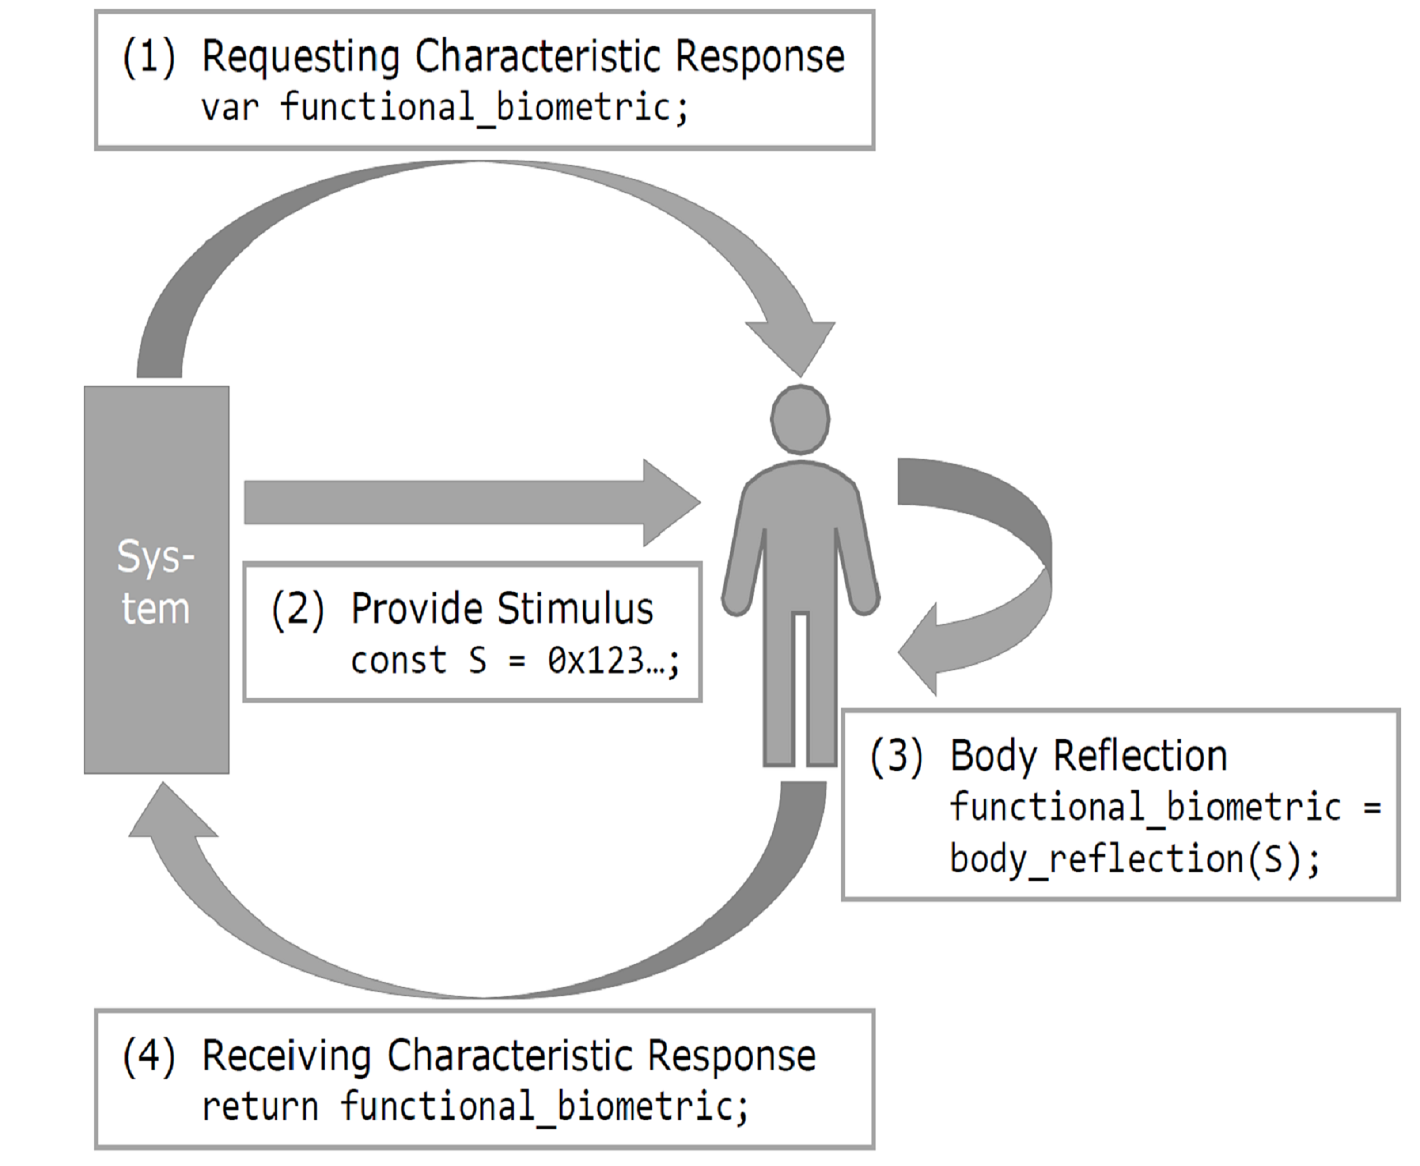
\includegraphics[width=0.4\textwidth]{biometric_funct.png}\label{fig:functBiom}}
	\end{center}
	\caption{(a) shows the authentication process of a traditional biometric system where a characteristic response is created based on someone's unique trait.
	(b) shows the order of steps for functional biometrics when a stimulus is added to create the characteristic based on body reflections \cite{schneegass2020functbiometric}.}
	\label{fig:biometricsVersions}
\end{figure}

In this category of biometric authentication the authentication system provides an additional stimulus during the enrolment phase.
This stimulus is applied to the individuals body where it gets modified and afterwards captured (cf.~Figure~\ref{fig:functBiom}).
Due to different personal biological characteristics the modification of the stimulus is unique for each combination of user and stimulus.
Requirements Schneegass et al. proposed are two hardware components in form of a Stimulus Generation Unit (SGU) and a Body Reflection Sensor (BRS).
These two have to be designed as a dependence of the underlying biometric trait. Exemplarily when sound is used as the stimulus the SGU will be most likely some kind of microphone and the BRS a speaker.
During the enrolment process described above stimulus and its transformation are saved as a secret two-tuple ($x, f(x)$) with $ x $ being the stimulus and $ f(x) $ the transformation.
Now when the related user wants to authenticate the stimulus is reapplied and it is expected to get $f(x)$ as response again.
An additional security measure provided by functional biometrics is that when the stimulus gets leaked or lost the system is not fully compromised because the stimulus is only an exchangeable medium.
The secret stems from the body reflection function which is unique to the user, unknown and hard to manipulate.


As already mentioned before the SkullConduct work by Schneegass et al. is one of the key influences to this work. Not just because it is one of the first realizations for functional biometrics but it also 
serves as a source of inspiration for this work.
Schneegass et al. implemented a biometric authentication system using eyewear computers (e.g. Google Glass).
Therefore they used the concept of bone conduction which is already frequently used by hearing aids. SkullConduct, in this case, uses the bone conduction speaker of the Google Glass to emit a sound sample against the wearers head.
The sample which gets transformed due to the unique nature of each individuals head is captured by the glasses integrated microphone.
Results of this study  indicate that with all tested users SkullConduct had a probability of around 97\% when it comes just to identify a correct user.
Test of the system as an authentication tool showed an Equal Error Rate (EER) of around 6.9\% in average but with significant drops the shorter the used sample gets (less than 1 second).

Other work on authentication via smart devices includes e.g. the works from A. Johnston et al. who implemented a smartwatch based authentication module that used gait recognition \cite{johnston2015smartwatch}.
They adapted from previous work of theirs where gyro- and acceleration-sensors of smart phones were used to develop authentication methods \cite{kwapisz2010cell}.
The main thought behind the proposed use of gait authentication on smartwatches is that their place of wearing/usage is more consistent than the one of a smart phone and therefore more advantageous.
Each participants dataset includes both data from gyro- and acceleration-sensor.
Tests in regard of both design types showed that the general performance of authentication is way higher in average than the one of identification (e.g. 97.2\% compared to 79.2\%).
Additionally the overall performances of the acceleration-sensor was higher than the gyro-sensor.
Conclusions Johnston et al. drew from their results were that it is possible to authenticate someone sufficient enough using a smartwatch but they propose not to use the system for something other than a multi-modal biometric system at its current level. 

\section{Concept}
Even though the technology of smart devices has become more popular over the last recent years it still does take some effort to protect them sufficiently in comparison to e.g. smartphones.
These smart devices need personal authentication because they can collect sensible data while in usage, could be used to display instant messages or can be used as a payment method with integrations of applications such as paypal or apple pay.
Possible solutions to solve this could be traditional authentication methods even though it can be tricky executing them since smart watches normally have very little displays whereas other smart devices could not even have a display on which a pin or security pattern could be entered.

An early example of using (smart)devices as an extra medium for authentication comes form Corner and Noble in their 2002 work "Zero-Interaction Authentication"\cite{corner2002zeroInt}.
There they provided an implicit decryption system for laptops which relies on a wearable token generator to implicitly generate and send the decryption keys when they are needed.
One example they proposed for the use as the token generator was an IBM Linux watch, an early 2000s predecessor from the nowadays smartwatch.

The introduction of behavioural biometrics showed alternatives to these previously describes methods.
Analysing e.g. the uniqueness of an individuals movements or other behaviour these biometric mechanisms do not rely on the use of knowledge based authenticators like the traditional methods.

Another alternative to these two types of authentication would be the use of the new approach on functional biometrics.
For example, a smartwatch based authentication system which uses functional biometrics could send a stimulus on an interval base whose alteration is compared to a previously stored default value.
The advantage of this functional approach against the behavioural one is that, even though both are implicit, movements or behaviours could still be mimicked whereas the transformation of the functional system is based on  someone's body structure e.g. the done density.

Possible stimuli could be sound patters which use either white noise, frequency changes or little melodies.
The stimulus can then be applied to the wearer on a regular base over the time the device is worn to ensure it is used by the correct user.
Also if the stimulus used gets leaked or corrupted otherwise a functional biometric system does not need to be recalibrated completely.
Since even the system itself does not really know the nature of the transformation function only a new stimulus and new sample data are needed.
\newpage
\section{Implementation}
\section{Evaluation}
\section{Conclusion}
